%%%%%%%%%%%%%%%%%%%%%%%%%%%%%%%%%%%%%%%%%%%%%%%%%%%%%%%%%%%%%%%%%%%%%%%%%%%%%%%%
\documentclass[twocolumn]{revtex4}

%%%%%%%%%%%%%%%%%%%%%%%%%%%%%%%%%%%%%%%%%%%%%%%%%%%%%%%%%%%%%%%%%%%%%%%%%%%%%%%%
% Note that comments begin with a "%" and are not turned into text in the .pdf
% document.
%%%%%%%%%%%%%%%%%%%%%%%%%%%%%%%%%%%%%%%%%%%%%%%%%%%%%%%%%%%%%%%%%%%%%%%%%%%%%%%%

%%%%%%%%%%%%%%%%%%%%%%%%%%%%%%%%%%%%%%%%%%%%%%%%%%%%%%%%%%%%%%%%%%%%%%%%%%%%%%%%
% Include some extra packages.
%%%%%%%%%%%%%%%%%%%%%%%%%%%%%%%%%%%%%%%%%%%%%%%%%%%%%%%%%%%%%%%%%%%%%%%%%%%%%%%%
\usepackage[]{graphicx}
%%%%%%%%%%%%%%%%%%%%%%%%%%%%%%%%%%%%%%%%%%%%%%%%%%%%%%%%%%%%%%%%%%%%%%%%%%%%%%%%

%%%%%%%%%%%%%%%%%%%%%%%%%%%%%%%%%%%%%%%%%%%%%%%%%%%%%%%%%%%%%%%%%%%%%%%%%%%%%%%%
\begin{document}

%%%%%%%%%%%%%%%%%%%%%%%%%%%%%%%%%%%%%%%%%%%%%%%%%%%%%%%%%%%%%%%%%%%%%%%%%%%%%%%%
\title{
Raptor's Food: Yes? Or No?
}

\author{D.~Wentworth}
\affiliation{Software Tools For Physicists Final Project}

\date{\today}
12/10/15

\begin{abstract}
	This project consisted of multiple questions with the ultimate goal to figure out whether or not a velociraptor will catch a person or if the person can outrun it. Furthermore, position and time was taken into account to determine when the velociraptor will catch the human. Continuing, the project asks to calculate the probability of the velociraptor biting the human. Ultimately, the motivation of this task is to test the skills and understanding of python notebook. The final result of the procedure was that roughly sixty two percent of the time the human would escape the velociraptor.
   \end{abstract}

\maketitle
%%%%%%%%%%%%%%%%%%%%%%%%%%%%%%%%%%%%%%%%%%%%%%%%%%%%%%%%%%%%%%%%%%%%%%%%%%%%%%%%
%%%%%%%%%%%%%%%%%%%%%%%%%%%%%%%%%%%%%%%%%%%%%%%%%%%%%%%%%%%%%%%%%%%%%%%%%%%%%%%%
\section{Problem One}
The problem stated to produce a position vs. time graph given humans run 3 meters per second and velociraptor run 18 meters per second while humans have a 30 meter head start. Also, acceleration is neglected.
\subsection{Python Notebook Process}
I began by creating my graph using numpy and matplotlib.pylab. For the graph the human velocity and the velociraptor velocity each were given a plot with 1001 points(1001 evenly spaced intervals are placed between 0 and 100). The graph shows the correlation between the velocities of the human and velociraptor, which always shows that the human has a head start of 30 meters at time 0 second
\subsection{Position vs. Time Graph}
\begin{figure}[ht]
\begin{center}
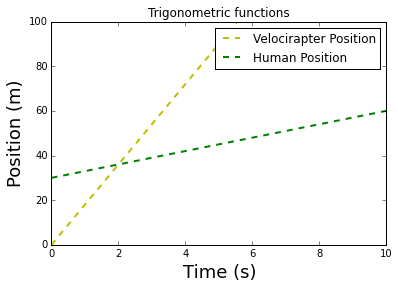
\includegraphics[scale=0.5]{Problem1_GraphImage.png}
\end{center}
\end{figure}
\subsection{Equations/Derivations}
These Derivations found the plots for the graphs.

x= np.linspace(0,10,1001)

Velociraptor:$$18(x)$$

Human:$$30+3(x)$$


%%%%%%%%%%%%%%%%%%%%%%%%%%%%%%%%%%%%%%%%%%%%%%%%%%%%%%%%%%%%%%%%%%%%%%%%%%%%%%%%
%%%%%%%%%%%%%%%%%%%%%%%%%%%%%%%%%%%%%%%%%%%%%%%%%%%%%%%%%%%%%%%%%%%%%%%%%%%%%%%%
\section{Problem Two}
The problem stated to locate both how far the human has run and how much time has elapsed.
\subsection{Python Notebook Process}
To solve the problem I used a for loop to take the range of the length of the variable "raptor" which would print the distance the human and the velociraptor traveled at the same time interval. Furthermore, I added an if statement to find the point at which the velociraptor caught up to the human. Once these numbers were found, I printed the distance the human traveled until the velociraptor caught up, also the distance at which the velociraptor travel until it caught up to the human. Finally, I also had the code print out the time elapsed until the velociraptor caught up to the human.
\section{Problem Three}
The problem stated to find out how much time has passed when the velociraptor is 1 meter away and how far the human has run when the velociraptor is 1 meter away.
\subsection{Python Notebook Process}
This setup is similar to the process in problem two, although I incorporated an if statement with two conditions to support when the velociraptor is 1 meter away. From here the velociraptor and human distances 1 meter away from each are found and recorded to the respected variables. Also, because of linspace the for statement I setup a range between 1 and 1.4 to guarantee correct values. Next 30 meters is subtracted from the human value to find the total distance the human has run. Time is found from the x-axis on the previous graph. Finally, the distance the human ran is found along with the distance the velociraptor is found when they are 1 meter apart from each other, time is recorded too. Next I setup the same position time graph as before, yet added another plot to graphically show the point at which the velociraptor is 1 meter away from the human. 
\subsection{Position vs. Time Graph (when 1 meter away)}
\begin{figure}[ht]
\begin{center}
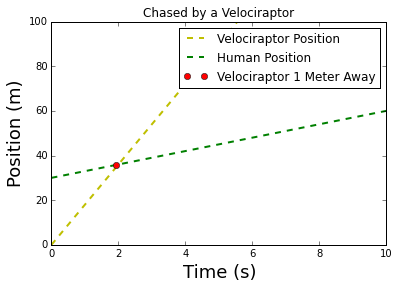
\includegraphics[scale=0.5]{Problem3_GraphImage.png}
\end{center}
\end{figure}
\subsection{Equations/Derivations}
$$1 = distanceHuman - distanceRaptor$$
\section{Problem Four}
The problem began by stating when the velociraptor is 1 meter away it bites and has a 20 percent chance the first time, 15 percent the second time it bites if missed the first, and finally a 7 percent chance of biting the human if missed the second attempt. Also if the human is bitten they die, the question asks what the probability of the human escaping is.
\subsection{Python Notebook Process}
I created a variable equal to the number of times I wanted to run the simulation with 1 million numbers. I used a for statement for this. Inside the statement, if statements ran random number through a series of tests first being the first bite from the velociraptor. If the random number was greater than 20 percent (.2), it moved to the second bite to see if the random number was greater than 15 percent (.15) Then if it passed the second test it moved to the third to undergo bite three. If the random number was greater than 7 percent (.07) it passed which would successfully allow the human to escape. After 1 million "tests" were ran the code I found the probability using a float.
\subsection{Equations/Derivations}
$$prob = (chance/pts)100$$

 %%%%%%%%%%%%%%%%%%%%%%%%%%%%%%%%%%%%%%%%%%%%%%%%%%%%%%%%%%%%%%%%%%%%%%%%%%%%%%%%

%%%%%%%%%%%%%%%%%%%%%%%%%%%%%%%%%%%%%%%%%%%%%%%%%%%%%%%%%%%%%%%%%%%%%%%%%%%%%%%%
\end{document}
%%%%%%%%%%%%%%%%%%%%%%%%%%%%%%%%%%%%%%%%%%%%%%%%%%%%%%%%%%%%%%%%%%%%%%%%%%%%%%%%
